\subsection{Pipelined Matrix Multiply}
If we look back at algorithm \ref{alg:matmul}, we may see that it is both embarrasingly parallel in that each of the loops with constant $i$ are totally independent.  Furthermore, the only computation is in the form of a multiply-accumulate operation which is an operation which FPGA hardware is already optimized for, and only requires one DSP slice.  So we may allocate some number of DSP slices to process the same number of inner products simultaneously.  Now, the Xilinx DSP48 slice is a fairly complicated component, and we do not require all of its functionality to accomplish this relatively simple task.  In order to simplify our design, we used one of Xilinx's IP cores, the Multiply Adder.  This component essentially provides multiply accumulate functionality in a simple package, the functional block diagram is shown in figure \ref{fig:mac}

\begin{figure}[H]
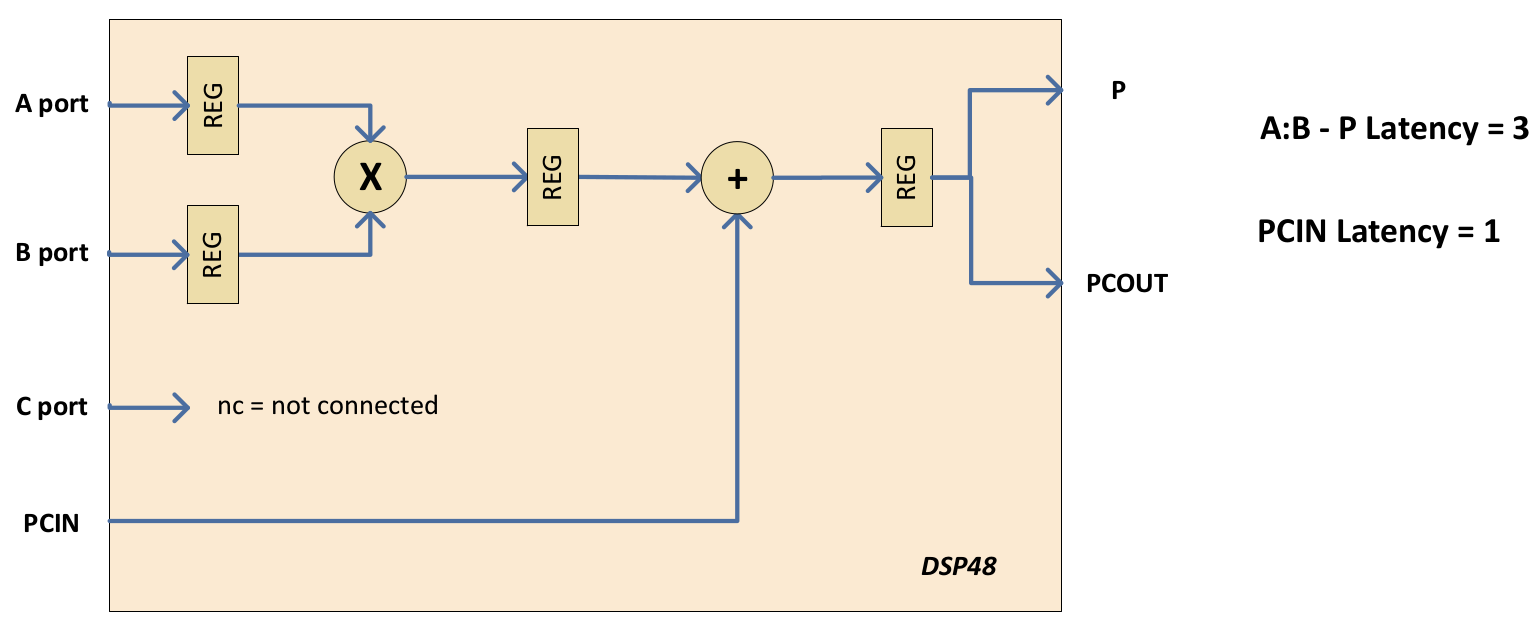
\includegraphics[width=\textwidth]{mac.png}
\caption{Functional diagram of the Multiply Adder}
\label{fig:mac}
\centering
\end{figure}

Connecting the output carry (PCOUT) to the output carry (PCIN) gives a multiply accumulate effect.  Note, however that the latency of the final output is now proportional to the size of the matrix.  More columns means the component will have to accumulate for a longer period of time.  If the amount of rows grows larger than the number of DSP slices we have, which is likely, the rows must be processed in sequence.  To allow for this, we also included a `programmable' state machine in our inner product component which clears the carry after a number of clock cycles indicated by an input signal.

We implemented the design and verified it for a simple test case of two vectors, as shown in figure \ref{fig:inner_product_verify}

\begin{figure}[H]
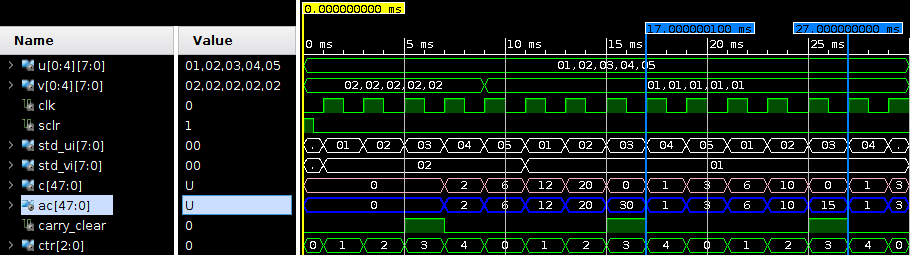
\includegraphics[width=\textwidth]{inner_product_verify.png}
\caption{The waveform of a simple inner product test.}
\label{fig:inner_product_verify}
\centering
\end{figure}

Note the delay of three clock cycles between the final input of the first vector and the final, correct value at the output of the inner product component, \verb|ac|.  The \verb|carry_clear| signal shown is driven by the programmable state machine, which is essentially just creating a signal with a period of 5 clock cycles, the length of the vectors being multiplied.  We will see that this design is useful for not only matrix multiplication, but convolution as well.




